\section{Massless Scalar Exchange\label{SecMasslessSca4}}
%%%%%%%%%%%%%%%%%%%%%%%%%%%%%%%%%%%%%%%%%%%%%%%%%%%%%%%%%%%%%%%%%%%%%%%%%%%%%%%%%%%%%%%%%
The starting point is a two-body path integral for two massive scalar particles $a$ and $b$ that are coupled to an external massless scalar field $\phi$,
\begin{equation}
	\mathcal{G}_{\phi}[\phi] = \int\limits_{x_{1}}^{x_{3}} \mathrm{D}q_{a}(\tau) \int\limits_{x_{2}}^{x_{4}} \mathrm{D}q_{b}(\sigma) \, \exp{\left(- i S_{P}[q_{a}, q_{b}, \phi] \right)}
\end{equation}
The particle action functional $S_{P}$ is
\begin{equation}
	S_{P}[q_{a}, q_{b}, \phi] \equiv S_{0}[q_{a}, q_{b}] + S_{\text{int}}[q_{a}, q_{b}, \phi]
\end{equation}
with the free term $S_{0}$ given by
\begin{equation}
	S_{0}\left[q_{a}, q_{b} \right] \equiv \int \mathrm{d}\tau \left[- \frac{1}{2} \dot{q}_{a}^{2} + \frac{1}{2} m^{2}_{a} \right] + \int \mathrm{d}\sigma \left[- \frac{1}{2} \dot{q}_{b}^{2} + \frac{1}{2} m^{2}_{b} \right] \label{FreeS}
\end{equation}
and the term with the coupling to the external field $\phi$ is given by
\begin{equation}
	S_{\text{int}}[q_{a}, q_{b}, \phi] \equiv \int \mathrm{d}\tau \, \phi[q_{a}(\tau)] + \int \mathrm{d}\sigma \, \phi[q_{b}(\sigma)] \label{SintSca}
\end{equation}
%(Note that we are working in the gauge where each worldline metric is set to unity.)
We integrate over the field $\phi$ in order to obtain the ``effective'' interacting two-body path integral, which we will call the \textbf{two-body quantum kernel}:
\begin{equation}
	\mathcal{F}_{\phi}(3,4|1,2) \equiv \int \mathrm{D}\phi(x) \, \mathcal{G}_{\phi}[\phi] \exp{\left( -i S_{\text{kin}}[\phi] \right)}
\end{equation}
The functional measure $\mathrm{D}\phi(x)$ is normalized such that
\begin{equation}
	\int \mathrm{D}\phi(x) \, \exp{\left( -i S_{\text{kin}}[\phi] \right)} = 1
\end{equation}
Since $\phi$ is a massless scalar field, the functional $S_{\text{kin}}$ is given by
\begin{equation}
	S_{\text{kin}}[\phi] \equiv \frac{1}{2g_{0}^{2}} \int \int \mathrm{d}x \mathrm{d}y \left[ \phi(x) K_{0}(x | y) \phi(y) \right] \label{SkinSca}
\end{equation}
with
\begin{equation}
	K_{0}(x | y) \equiv \delta(x - y) \left( - \frac{1}{2} \partial^{2} \right)
\end{equation}
and $g_{0}$ is a \textit{dimensionful} coupling parameter. In order to integrate over $\phi$, it is convenient to rewrite $S_{\text{int}}$ as
\begin{equation}
	S_{\text{int}}[q_{a}, q_{b}, \phi] = \int \mathrm{d}x \, J(x) \phi(x)
\end{equation}
with
\begin{equation}
	J(x) \equiv \int \mathrm{d}\tau \, \delta[x - q_{a}(\tau)] + \int \mathrm{d}\sigma \, \delta[x - q_{b}(\sigma)]
\end{equation}
After integrating over $\phi$, we find
\begin{equation}
	\mathcal{F}_{\phi}(3,4|1,2) = \int\limits_{x_{1}}^{x_{3}} \mathrm{D}q_{a}(\tau) \int\limits_{x_{2}}^{x_{4}} \mathrm{D}q_{b}(\sigma) \, \exp{\left(- i S_{\phi}[q_{a}, q_{b}] \right)}
\end{equation}
with
\begin{equation}
	S_{\phi}[q_{a}, q_{b}] \equiv S_{0}[q_{a}, q_{b}] - \frac{g_{0}^{2}}{2} \int \int \mathrm{d}x \mathrm{d}y \left[ J(x) G_{0}(x | y) J(y) \right] \label{SPhiJGJ}
\end{equation}
Here $G_{0}$ is the massless scalar Green function,
\begin{equation}
	G_{0}(x|y) \equiv [K_{0}(x|y)]^{-1}
\end{equation}
Using the explicit form of $J$ we find
\begin{equation}
	\frac{g_{0}^{2}}{2} \int \int \mathrm{d}x \mathrm{d}y \left[ J(x) G_{0}(x | y) J(y) \right] = S_{1}^{\phi}[q_{a}, q_{b}] + S_{2}^{\phi}[q_{a}, q_{b}] \label{JGJSca}
\end{equation}
with $S_{1}^{\phi}$ containing terms that connect a particle worldline to itself,
\begin{equation}
\begin{split}
	S_{1}^{\phi}[q_{a}, q_{b}] \equiv {}& \frac{g_{0}^{2}}{2} \int \int \mathrm{d}\tau_{1} \mathrm{d}\tau_{2} \, G_{0}\left[ q_{a}(\tau_{1}) | q_{a}(\tau_{2}) \right] \\
	&+ \frac{g_{0}^{2}}{2} \int \int \mathrm{d}\sigma_{1} \mathrm{d}\sigma_{2} \, G_{0}\left[ q_{b}(\sigma_{1}) | q_{b}(\sigma_{2}) \right]
\end{split}
\end{equation}
and $S_{2}^{\phi}$ containing a term that connects two different particle worldlines,
\begin{equation}
	S_{2}^{\phi}[q_{a}, q_{b}] \equiv g^{2}_{0} \int \int \mathrm{d}\tau \mathrm{d}\sigma \, G_{0} \left[ q_{a}(\tau) | q_{b}(\sigma) \right] \label{S2Sca}
\end{equation}
Thus, after the functional integral over $\phi$ is done, we find the action functional (\ref{SPhiJGJ}) for a system of interacting massive particles with one-body and two-body interaction terms where the massless scalar Green function
\begin{equation}
	G_{0}(x|y) = -i \Gamma\left( \frac{D-2}{2} \right) \left[ \frac{2}{(x - y)^{2}} \right]^{(D-2)/2}
\end{equation}
plays the role of an external potential. In what follows we will \textit{ignore} the contributions from the self-interactions.

We set $\hbar = 1$ and $c = 1$. This means that action functionals are dimensionless. In \S\ref{SecDimAn} we found that the coupling $g_{0}$ has units
\begin{equation}
	[g_{0}] = \left( \frac{6 - D}{2} \right) [\text{mass}]
\end{equation}
We are going to work in $D = 4$, where $g_{0}$ has units
\begin{equation}
	D = 4: \qquad [g_{0}] = [\text{mass}]
\end{equation}
and in $D = 3$, where $g_{0}$ has units
\begin{equation}
	D = 3: \qquad [g_{0}] = \frac{3}{2} [\text{mass}]
\end{equation}
In anticipation of infrared problems, we are going to use dimensional regularization. When we study the four-dimensional theory, we shall write
\begin{equation}
	g_{0}^{2} = \frac{\alpha_{0}}{2 \pi} \mu^{(4 - D)} \label{g2Sca}
\end{equation}
where both $\sqrt{\alpha_{0}}$ and $\mu$ have units of mass. Similarly, when we study the three-dimensional theory, we shall write
\begin{equation}
	g_{0}^{2} = \frac{\beta_{0}}{(2 \pi)^{3/2}} \mu^{(3 - D)} \label{g2ScaD3}
\end{equation}
where $\sqrt[3]{\beta_{0}}$ has units of mass.

In the eikonal JWKB approximation, the path integral in $\mathcal{F}_{\phi}$ is dominated by the eikonal paths
\begin{equation}
\begin{split}
	e_{a}(\tau) &= \frac{x_{1} + x_{3}}{2} + \left( \frac{\tau}{T_{a}} \right) (x_{3} - x_{1}), \qquad {- \frac{T_{a}}{2} < \tau < \frac{T_{a}}{2} } \\
	e_{b}(\sigma) &= \frac{x_{2} + x_{4}}{2} + \left( \frac{\sigma}{T_{b}} \right) (x_{4} - x_{2}), \qquad {- \frac{T_{b}}{2} < \sigma < \frac{T_{b}}{2} }
\end{split} \label{eikConf2}
\end{equation}
The two-body quantum kernel $\mathcal{F}_{\phi}$ becomes the \textbf{two-body semiclassical eikonal kernel},
\begin{equation}
	\mathcal{F}_{\phi}(3,4|1,2) \longrightarrow \mathcal{E}_{\phi}(3,4|
1,2) = \sqrt{-\det{(V_{\phi})}} \exp{\left( - i \Sigma_{\phi} \right)}
\end{equation}
where $\Sigma_{\phi}$ is given by
\begin{equation}
	\Sigma_{\phi} \equiv S_{\phi} \left[ e_{a}, e_{b} \right]
\end{equation}
and $V_{\phi}$ is
\begin{equation}
	V_{\phi} = \begin{pmatrix}
	V_{13} & V_{23} \\
	V_{14} & V_{24}
	\end{pmatrix}, \qquad V_{jk} \equiv -i \frac{\partial^{2} \Sigma_{\phi}}{\partial x_{j} \partial x_{k}}
\end{equation}
We now compute $\Sigma_{\phi}$ and $V_{\phi}$.
%%%%%%%%%%%%%%%%%%%%%%%%%%%%%%%%%%%%%%%%%%%%%%%%%%%%%%%%%%%%%%%%%%%%%%%%%%%%%%%%%%%%%%%%%
\subsection{Eikonal Van Vleck Function\label{EVVFun}}
%%%%%%%%%%%%%%%%%%%%%%%%%%%%%%%%%%%%%%%%%%%%%%%%%%%%%%%%%%%%%%%%%%%%%%%%%%%%%%%%%%%%%%%%%
The free part of the eikonal Van Vleck function is
\begin{align}
	\Sigma_{0} &\equiv S_{0}\left[ e_{a}, e_{b} \right] \nonumber \\
	&= -\frac{1}{2 T_{a}} (x_{3} - x_{1})^{2} + \frac{m_{a}^{2} T_{a}}{2} -\frac{1}{2 T_{b}} (x_{4} - x_{2})^{2} + \frac{m_{b}^{2} T_{b}}{2} \label{Sigma0}
\end{align}
After ignoring the self-interactions, the only contribution remaining is from the two-body interaction:
\begin{align}
	\Sigma_{2}^{\phi} &\equiv S_{2}^{\phi}\left[ e_{a}, e_{b} \right] \nonumber \\
	&= g^{2}_{0} \int \int \mathrm{d}\tau \mathrm{d}\sigma \, G_{0} \left[ e_{a}(\tau) | e_{b}(\sigma) \right] \nonumber \\
	&= -\frac{i \alpha_{0} \mu^{2}}{2 \pi} \Gamma\left( \frac{D - 2}{2} \right) \int \int \mathrm{d}\tau \mathrm{d}\sigma \left( \frac{2}{\mu^{2} \left[ e_{a}(\tau) - e_{b}(\sigma) \right]^{2}} \right)^{(D - 2)/2} \nonumber \\
	&= -\frac{i \alpha_{0} \mu^{2}}{2 \pi} \Upsilon \label{Sig2Phi}
\end{align}
where we have denoted
\begin{equation}
	\Upsilon \equiv \Gamma\left( \frac{D - 2}{2} \right) \int \int \mathrm{d}\tau \mathrm{d}\sigma \left( \frac{2}{\mu^{2} \left[ e_{a}(\tau) - e_{b}(\sigma) \right]^{2}} \right)^{(D - 2)/2} \label{upsi}
\end{equation}
We introduce a Schwinger parameter $T_{0}$ and rewrite $\Upsilon$ as
\begin{equation}
	\Upsilon = \int \int \mathrm{d}\tau \mathrm{d}\sigma \int\limits_{0}^{\infty} \mathrm{d}T_{0} \left( \frac{1}{T_{0}} \right)^{D/2} \exp{\left( -\frac{\mu^{2}}{2 T_{0}} \left[ e_{a}(\tau) - e_{b}(\sigma) \right]^{2} \right)} \label{Sigmaphi}
\end{equation}
With the eikonal paths (\ref{eikConf2}) we have
\begin{equation}
	e_{a}(\tau) - e_{b}(\sigma) = X_{12} + \left( \frac{\tau}{T_{a}} \right) x_{31} - \left( \frac{\sigma}{T_{b}} \right) x_{42}
\end{equation}
and thus
\begin{equation}
\begin{split}
	\left[ e_{a}(\tau) - e_{b}(\sigma) \right]^{2} = {}& X_{12}^{2} + 2 \left( X_{12} \cdot x_{31} \right) \left( \frac{\tau}{T_{a}} \right) - 2 \left( X_{12} \cdot x_{42} \right) \left( \frac{\sigma}{T_{b}} \right) \\
	&+ x_{31}^{2} \left( \frac{\tau}{T_{a}} \right)^{2} + x_{42}^{2} \left( \frac{\sigma}{T_{b}} \right)^{2} - 2 \left( x_{31} \cdot x_{42} \right) \left( \frac{\tau \sigma}{T_{a} T_{b}} \right)
\end{split}
\end{equation}
The variables $X_{12}$, $x_{31}$ and $x_{42}$ are defined below. The advantage of writing $\Sigma_{2}^{\phi}$ in the form (\ref{Sigmaphi}) is that the integrand becomes Gaussian. In the eikonal JWKB approximation, the separation between the two particles is always very large, compared to other distances in the problem. That is,
\begin{equation}
	{\left[ e_{a}(\tau) - e_{b}(\sigma) \right]^{2} \gg 0 }
\end{equation}
and thus we can use stationary methods to evaluate the integral over $(\tau, \sigma)$. The stationary point is
\begin{equation}
\begin{split}
	\tau_{*} &= -T_{a} \left[ \frac{x_{42}^{2} \left( X_{12} \cdot x_{31} \right) - \left( X_{12} \cdot x_{42} \right) \left( x_{31} \cdot x_{42} \right)}{ x_{31}^{2} x_{42}^{2} - \left( x_{31} \cdot x_{42} \right)^{2} } \right] \\
	\sigma_{*} &= +T_{b} \left[ \frac{x_{31}^{2} \left( X_{12} \cdot x_{42} \right) - \left( X_{12} \cdot x_{31} \right) \left( x_{31} \cdot x_{42} \right)}{ x_{31}^{2} x_{42}^{2} - \left( x_{31} \cdot x_{42} \right)^{2} } \right]
\end{split} \label{TauSigmaStar}
\end{equation}
At this stationary point, we find
\begin{equation}
\begin{split}
	B_{12} \equiv {}& e_{a}(\tau_{*}) - e_{b}(\sigma_{*}) \\
	= {}& X_{12} - \left[ \frac{x_{42}^{2} \left( X_{12} \cdot x_{31} \right) - \left( X_{12} \cdot x_{42} \right) \left( x_{31} \cdot x_{42} \right)}{ x_{31}^{2} x_{42}^{2} - \left( x_{31} \cdot x_{42} \right)^{2} } \right] x_{31} \\
	&- \left[ \frac{x_{31}^{2} \left( X_{12} \cdot x_{42} \right) - \left( X_{12} \cdot x_{31} \right) \left( x_{31} \cdot x_{42} \right)}{ x_{31}^{2} x_{42}^{2} - \left( x_{31} \cdot x_{42} \right)^{2} } \right] x_{42}
\end{split}
\end{equation}
The scalar $B_{12}^{2}$ corresponds to the minimum of the squared separation between the particles. Even though it is the minimum separation, by virtue of the eikonal approximation, $B_{12}^{2}$ is large compared to other distances in the problem. Note that the vector $B_{12}$ is orthogonal to any vector that is a linear combination of $x_{31}$ and $x_{42}$ (hence, $B_{12}$ has $D-2$ independent components). After integrating over $\tau$ and $\sigma$, we find
\begin{align}
	\Upsilon &\approx \frac{2 \pi}{\mu^{2}} \frac{T_{a} T_{b}}{\sqrt{x_{31}^{2} x_{42}^{2} - (x_{31} \cdot x_{42})^{2}}} \int\limits_{0}^{\infty} \mathrm{d}T_{0} \left( \frac{1}{T_{0}} \right)^{(D - 2)/2} \exp{\left( -\frac{\mu^{2}}{2 T_{0}} B_{12}^{2} \right)} \nonumber \\
	&= \frac{2 \pi}{\mu^{2}} \frac{T_{a} T_{b}}{\sqrt{x_{31}^{2} x_{42}^{2} - (x_{31} \cdot x_{42})^{2}}} \Gamma\left( \frac{D - 4}{2} \right) \left( \frac{2}{\mu^{2} B_{12}^{2}} \right)^{(D - 4)/2} \label{upsi2}
\end{align}
Thus, $\Sigma_{2}^{\phi}$ gives
\begin{equation}
	\Sigma_{2}^{\phi} \approx -i\alpha_{0} \left[ \frac{T_{a} T_{b}}{\sqrt{x_{31}^{2} x_{42}^{2} - (x_{31} \cdot x_{42})^{2}}} \right] \Gamma\left( \frac{D - 4}{2} \right) \left( \frac{2}{\mu^{2} B_{12}^{2}} \right)^{(D - 4)/2} \label{Sig2Phi2}
\end{equation}
Note that $\Sigma_{2}^{\phi}$ is proportional to a massless scalar propagator in $D - 2$ dimensions, and thus has the familiar divergence when $D - 2 = 2$, i.e. when $D = 4$. In order to simplify the equations we work with $D = 4 + 2 \epsilon$ and introduce
\begin{equation}
	\rho_{0} \equiv \frac{T_{a} T_{b}}{\sqrt{x_{31}^{2} x_{42}^{2} - (x_{31} \cdot x_{42})^{2}}} \label{rho0Def}
\end{equation}
such that we can simply write
\begin{equation}
	\Sigma_{2}^{\phi} \approx -i\alpha_{0} \rho_{0} \Gamma(\epsilon) \left( \frac{2}{\mu^{2} B_{12}^{2}} \right)^{\epsilon} \label{Sigmaphi2}
\end{equation}
The quantity $\rho_{0}$ has units of inverse mass squared and depends on the worldline moduli $T_{a}$ and $T_{b}$. The product $\alpha_{0} \rho_{0}$ is dimensionless.
%%%%%%%%%%%%%%%%%%%%%%%%%%%%%%%%%%%%%%%%%%%%%%%%%%%%%%%%%%%%%%%%%%%%%%%%%%%%%%%%%%%%%%%%%
\subsection{Eikonal Van Vleck Matrix\label{EVVMat}}
%%%%%%%%%%%%%%%%%%%%%%%%%%%%%%%%%%%%%%%%%%%%%%%%%%%%%%%%%%%%%%%%%%%%%%%%%%%%%%%%%%%%%%%%%
Since the Van Vleck function $\Sigma_{\phi}$ has the form $\Sigma_{\phi} = \Sigma_{0} - \Sigma_{2}^{\phi}$, we can write the Van Vleck matrix $V_{\phi}$ as $V_{\phi} = V_{0} - V_{2}^{\phi}$ with
\begin{equation}
	V_{0} = \begin{pmatrix}
	u_{13} & u_{23} \\
	u_{14} & u_{24}
	\end{pmatrix}, \qquad u_{jk} \equiv - i \frac{\partial^{2} \Sigma_{0}}{\partial x_{j} \partial x_{k}}
\end{equation}
and
\begin{equation}
	V_{2}^{\phi} = \begin{pmatrix}
	v_{13} & v_{23} \\
	v_{14} & v_{24}
	\end{pmatrix}, \qquad v_{jk} \equiv - i \frac{\partial^{2} \Sigma_{2}^{\phi}}{\partial x_{j} \partial x_{k}}
\end{equation}
The determinant of $V_{\phi}$ can be written as
\begin{equation}
	\det{(V_{\phi})} = \det{(V_{0} - V_{2}^{\phi})} = \det{(I - W)} \det{(V_{0})}, \qquad W \equiv V_{2}^{\phi}(V_{0})^{-1}
\end{equation}
Recall that
\begin{equation}
	\det{(I - W)} = \exp{\left[ - \sum_{n = 1}^{\infty} \frac{1}{n} \operatorname{tr}{(W^{n})} \right]}
\end{equation}
Hence, the square root of the Van Vleck determinant is
\begin{equation}
	\sqrt{- \det{(V_{\phi})}} = \sqrt{- \det{(V_{0})}} \exp{\left[ - \sum_{n = 1}^{\infty} \frac{1}{2n} \operatorname{tr}{(W^{n})} \right]} \label{FullVVDet}
\end{equation}
Using (\ref{Sigma0}) it is easy to show that
\begin{equation}
\begin{split}
	(u_{13})_{mn} = \left(- \frac{i}{T_{a}} \right) \eta_{mn}, &\qquad (u_{23})_{mn} = 0 \\
	(u_{14})_{mn} = 0, &\qquad (u_{42})_{mn} = \left(- \frac{i}{T_{b}} \right) \eta_{mn}
\end{split} \label{uMats}
\end{equation}
and thus
\begin{equation}
	\sqrt{- \det{(V_{0})}} = \left(- \frac{i}{T_{a}} \right)^{D/2} \left(- \frac{i}{T_{b}} \right)^{D/2} \label{DetV0}
\end{equation}
Just like in the nonrelativistic case, we will \textit{ignore} all the contributions from the matrix $W$. If we compute $W$, we find that all the contributions from the traces of powers of $W$ involve powers of $B_{12}^{2}$ that are less (i.e. more negative) than the power in $\Sigma_{2}^{\phi}$. Thus, in the eikonal JWKB approximation, the leading term with $B_{12}^{2}$ inside the exponential comes from $\Sigma_{2}$ and we can ignore all contributions from $W$. That is,
\begin{equation}
	\sqrt{- \det{(V_{\phi})}} \approx \sqrt{- \det{(V_{0})}} \label{DetV}
\end{equation}
%%%%%%%%%%%%%%%%%%%%%%%%%%%%%%%%%%%%%%%%%%%%%%%%%%%%%%%%%%%%%%%%%%%%%%%%%%%%%%%%%%%%%%%%%
\subsection{Eikonal S-Matrix\label{SMatrixMasslessSca}}
%%%%%%%%%%%%%%%%%%%%%%%%%%%%%%%%%%%%%%%%%%%%%%%%%%%%%%%%%%%%%%%%%%%%%%%%%%%%%%%%%%%%%%%%%
At this stage we have everything we need to build the two-body semiclassical eikonal kernel:
\begin{equation}
	\mathcal{E}_{\phi}(3,4|1,2) = \sqrt{- \det{(V_{\phi})}} \exp{\left( - i \Sigma_{\phi} \right)}
\end{equation}
Using (\ref{Sigma0}), (\ref{Sigmaphi2}), (\ref{DetV}) and (\ref{DetV0}) we find
\begin{equation}
	\mathcal{E}_{\phi}(3,4|1,2) \approx \left(- \frac{i}{T_{a}} \right)^{D/2} \left(- \frac{i}{T_{b}} \right)^{D/2} \left[ -1 + \exp{\left(i \Sigma_{2}^{\phi} \right)} \right] \exp{\left(-i \Sigma_{0} \right)} \label{EPhi3412}
\end{equation}
where we have subtracted the disconnected part. We write the factor inside square brackets as an infinite series:
\begin{equation}
	{-1} + \exp{\left(i \Sigma_{2}^{\phi} \right)} = \sum_{l = 1}^{\infty} \frac{\left( \alpha_{0} \rho_{0} \right)^{l}}{\Gamma(l + 1)} [\Gamma(\epsilon)]^{l} \left( \frac{2}{\mu^{2} B_{12}^{2}} \right)^{l \epsilon} 
\end{equation}
This expression provides a way to understand the meaning of the semiclassical eikonal kernel $\mathcal{E}_{\phi}$: The $l$-th term in the sum contains the product of $l$ massless scalar propagators in $D - 2$ dimensions, with each propagator connecting the \textit{same} two points with separation vector $B_{12}$. The quantum kernel corresponds to the sum over ladder and crossed ladder contributions. We see that in the semiclassical JWKB approximation, the ladder and crossed ladder contributions are contracted along the $s$-channel direction and yield the semiclassical eikonal kernel. For example, at the 1-loop level we have the eikonal contraction of the box,
\begin{equation}
	\vcenter{\hbox{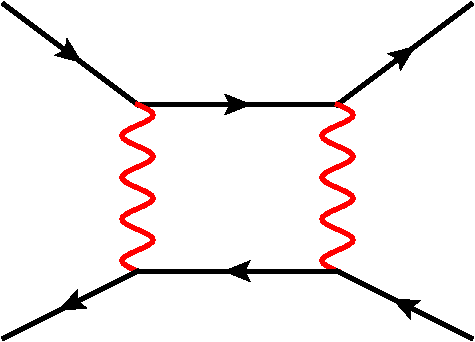
\includegraphics[scale=0.4]{Figures/1Box.pdf}}} \quad \longrightarrow \quad \vcenter{\hbox{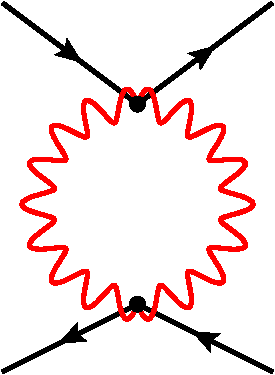
\includegraphics[scale=0.4]{Figures/1Eikonal.pdf}}}
\end{equation}
This is different to what happens in the Regge limit ($|t| \rightarrow \infty$), where the contraction is along the $t$-channel,
\begin{equation}
	\vcenter{\hbox{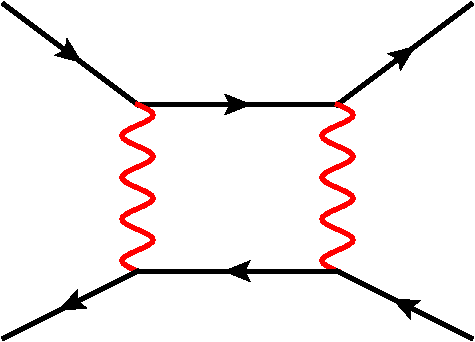
\includegraphics[scale=0.4]{Figures/1Box.pdf}}} \quad \longrightarrow \quad \vcenter{\hbox{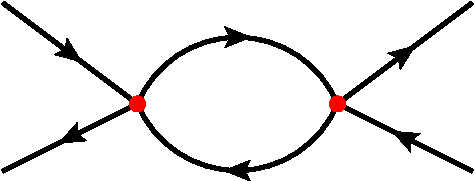
\includegraphics[scale=0.4]{Figures/1Regge.pdf}}}
\end{equation}
Similarly, at the 2-loops level, the eikonal contraction of the double box is
\begin{equation}
	\vcenter{\hbox{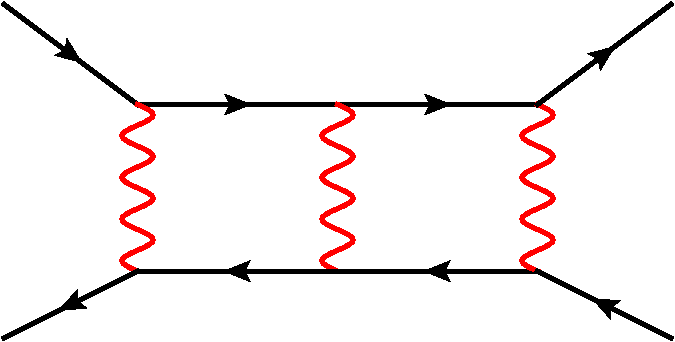
\includegraphics[scale=0.4]{Figures/2Box.pdf}}} \quad \longrightarrow \quad \vcenter{\hbox{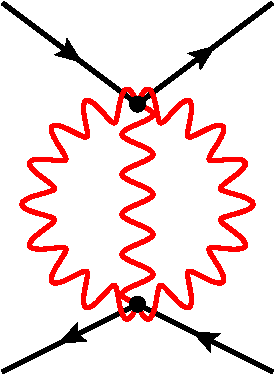
\includegraphics[scale=0.4]{Figures/2Eikonal.pdf}}}
\end{equation}
which is different from the Regge contraction,
\begin{equation}
	\vcenter{\hbox{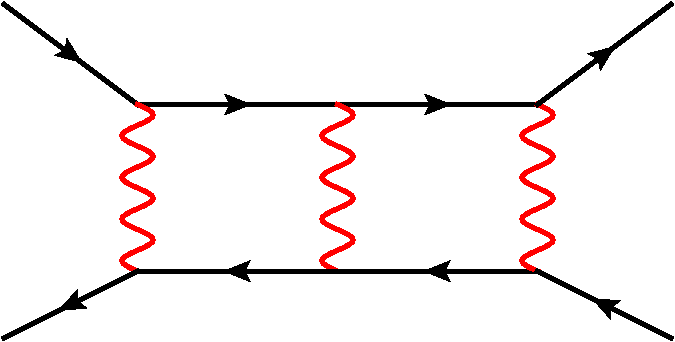
\includegraphics[scale=0.4]{Figures/2Box.pdf}}} \quad \longrightarrow \quad \vcenter{\hbox{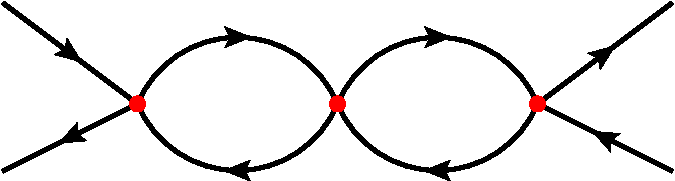
\includegraphics[scale=0.4]{Figures/2Regge.pdf}}}
\end{equation}
Of course, we do not expect agreement in the first place, since the eikonal approximation involves $t \rightarrow 0$, while the Regge limit involves $|t| \rightarrow \infty$.

With $\mathcal{E}_{\phi}$ in hand, we compute the \textbf{un-integrated semiclassical eikonal S-matrix},
\begin{equation}
	\mathcal{S}_{\phi}(3, 4|1, 2) \approx \int \int \int \int \mathrm{d}x_{1}\mathrm{d}x_{2}\mathrm{d}x_{3}\mathrm{d}x_{4} \, \overline{\mathcal{W}}_{O}(3, 4) \mathcal{W}_{I}(1, 2) \mathcal{E}_{\phi}(3, 4|1, 2) \label{UnIntegratedSca}
\end{equation}
where, for the two-body system, we have
\begin{align}
	\mathcal{W}_{I}(1, 2) &= \exp{\left[ \frac{i T_{a}}{4}  \left( p_{1}^{2} + m_{1}^{2} \right) + \frac{i T_{b}}{4} \left( p_{2}^{2} + m_{2}^{2} \right) + i x_{1} \cdot p_{1} + i x_{2} \cdot p_{2} \right]} \\
	\overline{\mathcal{W}}_{O}(3, 4) &= \exp{\left[ \frac{i T_{a}}{4} \left( p_{3}^{2} + m_{3}^{2} \right) + \frac{i T_{b}}{4} \left( p_{4}^{2} + m_{4}^{2} \right) -i x_{3} \cdot p_{3} - i x_{4} \cdot p_{4} \right]}
\end{align}
Then we compute the \textbf{integrated semiclassical eikonal S-matrix}:
\begin{equation}
	\mathcal{A}_{\phi}(3,4|1,2) \approx \int\limits_{0}^{\infty} \mathrm{d}T_{a} \int\limits_{0}^{\infty} \mathrm{d}T_{b} \, \mathcal{S}_{\phi}(3,4|1,2) \label{IntegratedSca}
\end{equation}
%The four limits in (\ref{IntegratedSca}) set
%\begin{equation}
%	\tau_{I} = {- \frac{T_{a}}{2} }, \qquad \sigma_{I} = {- \frac{T_{b}}{2} }, \qquad \tau_{O} = {+ \frac{T_{a}}{2} }, \qquad \sigma_{O} = {+ \frac{T_{b}}{2} }
%\end{equation}
%Thus,
%\begin{equation}
%	\Delta \tau = \tau_{O} - \tau_{I} = T_{a}, \qquad \Delta \sigma = \sigma_{O} - \sigma_{I} = T_{b}
%\end{equation}
We will evaluate the integration over $T_{a}$ and $T_{b}$ later.

In order to perform the integration in (\ref{UnIntegratedSca}) we first make a change of variables, and also introduce corresponding conjugate momenta:
\begin{equation}
\begin{split}
	X \equiv \frac{x_{1} + x_{2} + x_{3} + x_{4}}{4} &\qquad P \equiv p_{4} + p_{3} - p_{2} - p_{1} \\
	X_{12} \equiv \frac{x_{1} - x_{2} + x_{3} - x_{4}}{2} &\qquad P_{12} \equiv \frac{p_{3} - p_{1} + p_{2} - p_{4}}{2} \\
	x_{31} \equiv x_{3} - x_{1} &\qquad p_{31} \equiv \frac{p_{1} + p_{3}}{2} \\
	x_{42} \equiv x_{4} - x_{2} &\qquad p_{42} \equiv \frac{p_{2} + p_{4}}{2}
\end{split}
\end{equation}
such that
\begin{equation}
	x_{1} \cdot p_{1} + x_{2} \cdot p_{2} - x_{3} \cdot p_{3} - x_{4} \cdot p_{4} = - X \cdot P - X_{12} \cdot P_{12} - x_{31} \cdot p_{31} - x_{42} \cdot p_{42}
\end{equation}
Note that
\begin{equation}
	p_{1}^{2} + p_{3}^{2} = \frac{1}{8} \left(2 P_{12} + P \right)^{2} + 2 p_{31}^{2}, \qquad p_{2}^{2} + p_{4}^{2} = \frac{1}{8} \left(2 P_{12} - P \right)^{2} + 2 p_{42}^{2}
\end{equation}
These two identities allow us to write
\begin{equation}
\begin{split}
	\overline{\mathcal{W}}_{O} \mathcal{W}_{I} = {}& \exp{\left[ -i x_{31} \cdot p_{31} -i x_{42} \cdot p_{42} - i X \cdot P -i X_{12} \cdot P_{12} \right]} \\
	&\times \exp{\left[ \frac{i T_{a}}{2} p_{31}^{2} + \frac{i T_{a}}{32} \left(2 P_{12} + P \right)^{2} + \frac{i T_{a}}{4} (m_{1}^{2} + m_{3}^{2}) \right]} \\
	&\times \exp{\left[ \frac{i T_{b}}{2} p_{42}^{2} + \frac{i T_{b}}{32} \left(2 P_{12} - P \right)^{2} + \frac{i T_{b}}{4} (m_{2}^{2} + m_{4}^{2}) \right]} \\
	%&\times \exp{\left[ \frac{i T_{a}}{4} (m_{1}^{2} + m_{3}^{2}) + \frac{i T_{b}}{4} (m_{2}^{2} + m_{4}^{2}) \right]}
\end{split}
\end{equation}
Since $\mathcal{E}_{\phi}$ has no dependence on $X$, integration yields a Dirac delta:
\begin{equation}
	\int \mathrm{d}X \, \exp{\left(- i X \cdot P \right)} = \delta(P)
\end{equation}
This Dirac delta imposes the constraint $P = 0$, which leads to
\begin{equation}
	p_{1} + p_{2} = p_{3} + p_{4}
\end{equation}
We find that the total external momentum is conserved. This is one of the requirements for the external momenta to be physical. Using $P = 0$, we find
\begin{equation}
	P_{12} = p_{3} - p_{1} = p_{2} - p_{4}
\end{equation}
That is, $P_{12}$ measures the momentum transfer between the particles:
\begin{equation}
	t = {-P^{2}_{12}} = -(p_{1} - p_{3})^{2}
\end{equation}
Thus, after integrating over $X$, and using $P = 0$, we obtain
\begin{equation}
\begin{split}
	\overline{\mathcal{W}}_{O} \mathcal{W}_{I} = {}& \exp{\left[ -i x_{31} \cdot p_{31} -i x_{42} \cdot p_{42} -i X_{12} \cdot P_{12} \right]} \\
	&\times \exp{\left[ \frac{i T_{a}}{2} p_{31}^{2} + \frac{i T_{b}}{2} p_{42}^{2} \right]} \\
	&\times \exp{\left[ \frac{i T_{a}}{4} \left(m_{1}^{2} + m_{3}^{2} - \frac{t}{2} \right) + \frac{i T_{b}}{4} \left(m_{2}^{2} + m_{4}^{2} - \frac{t}{2} \right) \right]}
\end{split} \label{step1}
\end{equation}

Next we tackle the integration over $x_{31}$ and $x_{42}$. The exact integration is non-trivial because $\rho_{0}$ is a function of $x_{31}$ and $x_{42}$. We make another change of variables:
\begin{equation}
	x_{31} = T_{a} k_{31}, \qquad x_{42} = T_{b} k_{42}
\end{equation}
From dimensional analysis we expect $k_{31}$ and $k_{42}$ to have units of mass. In terms of $k_{31}$ and $k_{42}$, we have
\begin{equation}
	\rho_{0} = \frac{1}{\sqrt{k_{31}^{2} k_{42}^{2} - (k_{31} \cdot k_{42})^{2}}}
\end{equation}
which does not explicitly depend on the moduli $T_{a}$ and $T_{b}$. In terms of these new variables we have
\begin{equation}
\begin{split}
	\overline{\mathcal{W}}_{O} \mathcal{W}_{I} \exp{\left( -i \Sigma_{0} \right)} = {}& \exp{\left[ \frac{i T_{a}}{2} \left( k_{31} - p_{31} \right)^{2} + \frac{i T_{b}}{2} \left( k_{42} - p_{42} \right)^{2} \right]} \\
	&\times \exp{\left[ \frac{i T_{a}}{4} \left(m_{1}^{2} + m_{3}^{2} - 2 m_{a}^{2} - \frac{t}{2} \right) \right]} \\
	&\times \exp{\left[ \frac{i T_{b}}{4} \left(m_{2}^{2} + m_{4}^{2} - 2 m_{b}^{2} - \frac{t}{2} \right) \right]} \\
	&\times \exp{\left( - i X_{12} \cdot P_{12} \right)}
\end{split} \label{UFUI}
\end{equation}
The integrand in $(k_{31}, k_{42})$ is of the form ``Gaussian $\times$ function''. The Gaussian part is the first line in (\ref{UFUI}). At this stage we use stationary methods to evaluate the integral. The stationary point is
\begin{equation}
	\bar{k}_{31} = p_{31}, \qquad \bar{k}_{42} = p_{42}
\end{equation}
At this stationary point $\rho_{0}$ becomes a function of the external momenta,
\begin{equation}
	\rho_{0} = \frac{1}{\sqrt{p_{31}^{2} p_{42}^{2} - (p_{31} \cdot p_{42})^{2}}}
\end{equation}

The integral over $X_{12}$ remains:
\begin{equation}
\begin{split}
	\mathcal{A}_{\phi} = \delta(P) \int\limits_{0}^{\infty} \mathrm{d}T_{a} \int\limits_{0}^{\infty} \mathrm{d}T_{b} {}& \int \mathrm{d}X_{12} \left[ \sum_{l = 1}^{\infty} \frac{\left(\alpha_{0} \rho_{0} \right)^{l}}{\Gamma(l + 1)} [\Gamma(\epsilon)]^{l} \left(\frac{2}{\mu^{2} B_{12}^{2}} \right)^{l \epsilon} \right] \\
	&\times \exp{\left[ \frac{i T_{a}}{4} \left(m_{1}^{2} + m_{3}^{2} - 2 m_{a}^{2} - \frac{t}{2} \right) \right]} \\
	&\times \exp{\left[ \frac{i T_{b}}{4} \left(m_{2}^{2} + m_{4}^{2} - 2 m_{b}^{2} - \frac{t}{2} \right) \right]} \\
	&\times \exp{\left(- i X_{12} \cdot P_{12} \right)}
\end{split} \label{IntX12}
\end{equation}
Earlier we defined $B_{12}$ as the part of $X_{12}$ that is orthogonal to any linear combination of the vectors $x_{31}$ and $x_{42}$. But the net result of the integration over $x_{31}$ and $x_{42}$ was to replace $x_{31}$ by $ T_{a} p_{31}$ and $x_{42}$ by $ T_{b} p_{42}$. So we now write
\begin{equation}
	X_{12} = B_{12} + T_{a} b_{31} p_{31} + T_{b} b_{42} p_{42} \qquad B_{12} \cdot p_{31} = 0 \qquad B_{12} \cdot p_{42} = 0
\end{equation}
The volume element becomes
\begin{equation}
	\mathrm{d}X_{12} = T_{a} T_{b} \sqrt{p_{31}^{2} p_{42}^{2} - (p_{31} \cdot p_{42})^{2}} \mathrm{d}B_{12} \mathrm{d}b_{31} \mathrm{d}b_{42}
\end{equation}
which can be rewritten in terms of $\rho_{0}$,
\begin{equation}
	\mathrm{d}X_{12} = \alpha_{0} T_{a} T_{b} \left( \frac{1}{\alpha_{0} \rho_{0}} \right) \mathrm{d}B_{12} \mathrm{d}b_{31} \mathrm{d}b_{42} \label{dX12Sca}
\end{equation}
Note that
\begin{equation}
	X_{12} \cdot P_{12} = B_{12} \cdot P_{12} + T_{a} b_{31} (p_{31} \cdot P_{12}) + T_{b} b_{42} (p_{42} \cdot P_{12})
\end{equation}
Integration over $b_{31}$ and $b_{42}$ yields two Dirac deltas:
\begin{align}
	\int \mathrm{d}b_{31} \, \exp{\left[- i T_{a} b_{31} (p_{31} \cdot P_{12}) \right]} &= \frac{1}{T_{a}} \delta(p_{31} \cdot P_{12}) \\
	\int \mathrm{d}b_{42} \, \exp{\left[- i T_{b} b_{42} (p_{42} \cdot P_{12}) \right]} &= \frac{1}{T_{b}}  \delta(p_{42} \cdot P_{12})
\end{align}
These two Dirac deltas impose constraints that will be discussed later. At this stage the only part of the amplitude that depends on $T_{a}$ and $T_{b}$ is the second and third exponential factors in (\ref{IntX12}). Performing the integration over $T_{a}$ and $T_{b}$ yields
\begin{equation}
\begin{split}
	\int\limits_{0}^{\infty} \mathrm{d}T_{a} \, \exp{\left[ \frac{i T_{a}}{4} \left(m_{1}^{2} + m_{3}^{2} - 2 m_{a}^{2} - \frac{t}{2} \right) \right] } &= \frac{8i}{2 m_{1}^{2} + 2 m_{3}^{2} - 4 m_{a}^{2} - t} \\
	\int\limits_{0}^{\infty} \mathrm{d}T_{b} \, \exp{\left[ \frac{i T_{b}}{4} \left(m_{2}^{2} + m_{4}^{2} - 2 m_{b}^{2} - \frac{t}{2} \right) \right]} &= \frac{8i}{2 m_{2}^{2} + 2 m_{4}^{2} - 4 m_{b}^{2} - t}
\end{split} \label{IntTaTbTrunc}
\end{equation}

The last thing remaining is the integral over $B_{12}$:
\begin{equation}
\begin{split}
	\mathcal{A}_{\phi} = {}& \alpha_{0} \mathcal{N} \delta(P) \\
	&\times \int \mathrm{d}B_{12} \left[ \sum_{l = 1}^{\infty} \frac{\left(\alpha_{0} \rho_{0} \right)^{(l - 1)}}{\Gamma(l + 1)} [\Gamma(\epsilon)]^{l} \left(\frac{2}{\mu^{2} B_{12}^{2}} \right)^{l \epsilon} \right] \exp{\left( - i B_{12} \cdot P_{12} \right)}
\end{split} \label{IntB12}
\end{equation}
where we have collected many terms into
\begin{equation}
	\mathcal{N} \equiv \frac{(8i)^{2} \delta(p_{31} \cdot P_{12}) \delta(p_{42} \cdot P_{12})}{\left( 2 m_{1}^{2} + 2 m_{3}^{2} - 4 m_{a}^{2} - t \right) \left( 2 m_{2}^{2} + 2 m_{4}^{2} - 4 m_{b}^{2} - t \right)}
\end{equation}
In $D = 4 + 2 \epsilon$ dimensions the integral over $B_{12}$ is over $D - 2 = 2 + 2 \epsilon$ dimensions. After integrating over $B_{12}$ we find
\begin{equation}
\begin{split}
	\mathcal{A}_{\phi}(3,4|1,2) = {}& \alpha_{0} \mathcal{N} \delta(P) \left(\frac{1}{\mu^{2}} \right)^{(1 + \epsilon)} \\
	&\times \sum_{l = 1}^{\infty} \frac{\left(\alpha_{0} \rho_{0} \right)^{(l - 1)}}{\Gamma(l + 1)} \frac{[\Gamma(\epsilon)]^{l} \Gamma(1 + \epsilon - l \epsilon)}{\Gamma(l \epsilon)} \left(\frac{2\mu^{2}}{P_{12}^{2}} \right)^{(1 + \epsilon - l \epsilon)}
\end{split}
\end{equation}
which can be written as
\begin{equation}
\begin{split}
	\mathcal{A}_{\phi}(3,4|1,2) = {}& {-\frac{2\alpha_{0}}{t}} \mathcal{N} \delta(P) \left( \frac{1}{\mu^{2}} \right)^{\epsilon} \\
	&\times \sum_{L = 0}^{\infty} \frac{\left(\alpha_{0} \rho_{0} \right)^{L}}{\Gamma(L + 1)} \frac{\Gamma(1 + \epsilon) [\Gamma(\epsilon)]^{L} \Gamma(1 - L \epsilon)}{\Gamma(1 + \epsilon + L \epsilon)} \left( -\frac{t}{2 \mu^{2}} \right)^{L \epsilon}
\end{split}
\end{equation}
where we have used $t = - P_{12}^{2}$.

Before we put the external momenta on-shell (and thus make the external momenta \textit{physical}), we need to truncate from $\mathcal{A}_{\phi}$ the part that is divergent on-shell. Traditionally, truncation involves multiplying the amplitude by a product of inverse propagators $(p_{j}^{2} + m_{j}^{2})$ and then taking the limit $p_{j}^{2} \rightarrow - m_{j}^{2}$. Since we have four external states, we need to multiply $\mathcal{A}_{\phi}$ by four inverse propagators. The factor $\mathcal{N}$ is the product of four terms, each with units of inverse mass squared. On-shell, we must have
\begin{equation}
	p_{j}^{2} = - m_{j}^{2}, \qquad m_{1} = m_{3} = m_{a}, \qquad m_{2} = m_{4} = m_{b}
\end{equation}
The two one-dimensional Dirac deltas in $\mathcal{N}$ impose the constraints
\begin{equation}
	p_{31} \cdot P_{12} = \frac{p_{3}^{2} - p_{1}^{2}}{2} = 0, \qquad p_{42} \cdot P_{12} = \frac{p_{2}^{2} - p_{4}^{2}}{2} = 0
\end{equation}
These two constraints are satisfied on-shell. Thus, on-shell, we have
\begin{equation}
	\delta(p_{31} \cdot P_{12}) \rightarrow \infty, \qquad \delta(p_{42} \cdot P_{12}) \rightarrow \infty
\end{equation}
The two factors in the denominator of $\mathcal{N}$ vanish on-shell because, in the eikonal JWKB approximation, we have $m_{a}^{2} \gg t$ and $m_{b}^{2} \gg t$. Hence, we will argue that the net result of truncation and taking the on-shell limit is to eliminate $\mathcal{N}$ from $\mathcal{A}_{\phi}$. Thus, the \textit{truncated on-shell} scattering amplitude $\widehat{\mathcal{A}}_{\phi}$ is given by
\begin{align}
	\widehat{\mathcal{A}}_{\phi} &\equiv \left( \frac{\mu^{2\epsilon}}{\mathcal{N}} \right) \mathcal{A}_{\phi}(3, 4|1,2) \nonumber \\
	&= -\frac{2\alpha_{0}}{t} \delta(P) \left[ \sum_{L = 0}^{\infty} \frac{\left(\alpha_{0} \rho_{0} \right)^{L}}{\Gamma(L + 1)} \frac{\Gamma(1 + \epsilon) [\Gamma(\epsilon)]^{L} \Gamma(1 - L \epsilon)}{\Gamma(1 + \epsilon + L \epsilon)} \left( -\frac{t}{2 \mu^{2}} \right)^{L \epsilon} \right] \label{AHatPhi}
\end{align}
We can recognize the pre-factor as the tree-level amplitude for the exchange of a massless scalar,
\begin{equation}
	\mathcal{A}_{\text{tree}}^{\phi}(t) = -\frac{2\alpha_{0}}{t} \delta(P)
\end{equation}

Before we move on to a more explicit discussion of the different terms in the sum in (\ref{AHatPhi}), we briefly discuss $\rho_{0}$. Recall that
\begin{equation}
	\rho_{0} = \frac{1}{\sqrt{p_{31}^{2} p_{42}^{2} - (p_{31} \cdot p_{42})^{2}}}
\end{equation}
On-shell, we have
\begin{equation}
	p_{31}^{2} = \frac{t - 4 m_{a}^{2}}{4} \qquad p_{42}^{2} = \frac{t - 4 m_{b}^{2}}{4} \qquad p_{31} \cdot p_{42} = \frac{m_{a}^{2} + m_{b}^{2} - s}{2} - \frac{t}{4}
\end{equation}
Using
\begin{equation}
	s + t + u = 2m_{a}^{2} + 2m_{b}^{2}
\end{equation}
we can write
\begin{equation}
	p_{31}^{2} = \frac{2m_{b}^{2} - 2m_{a}^{2} - s - u}{4} \qquad p_{42}^{2} = \frac{2m_{a}^{2} - 2m_{b}^{2} - s - u}{4}
\end{equation}
and
\begin{equation}
	p_{31} \cdot p_{42} = \frac{u - s}{4}
\end{equation}
Thus,
\begin{equation}
	\rho_{0}(s, u) = \frac{2}{\sqrt{s u - (m_{a} + m_{b})^{2} (m_{a} - m_{b})^{2}}} \label{rho0su}
\end{equation}
In terms of $s$ and $t$, we have
\begin{equation}
	\rho_{0}(s, t) = \frac{2}{\sqrt{[s - (m_{a} - m_{b})^{2}] [(m_{a} + m_{b})^{2} - s] - s t}} \label{rho0st}
\end{equation}
or in terms of $t$ and $u$,
\begin{equation}
	\rho_{0}(t, u) = \frac{2}{\sqrt{[u - (m_{a} - m_{b})^{2}] [(m_{a} + m_{b})^{2} - u] - t u}} \label{rho0tu}
\end{equation}
Note that $s$ and $u$ appear in the same way in (\ref{rho0st}) and (\ref{rho0tu}). Also, (\ref{rho0su}) is symmetric under $s \longleftrightarrow u$.
%The cosine of the scattering angle $\theta_{s}$ is
%\begin{equation}
%	z_{s} \equiv \cos{(\theta_{s})} = 1 - \frac{2 s t}{[s - (m_{a} - m_{b})^{2}] [(m_{a} + m_{b})^{2} - s]}
%\end{equation}
%Writing $\rho_{0}$ in terms of $s$ and $z_{s}$ gives
%\begin{equation}
%	\rho_{0}(s, z_{s}) = \frac{2}{\sqrt{[s - (m_{a} - m_{b})^{2}] [(m_{a} + m_{b})^{2} - s]}} \sqrt{\frac{2}{1 + z_{s}}}
%\end{equation}
%Another way of writting $\rho_{0}$ is
%\begin{equation}
%	\rho_{0}(s, t, z) = \frac{2 m_{a} m_{b}}{\sqrt{s t}} \sqrt{\frac{1 - z}{1 + z}}
%\end{equation}
%In the eikonal approximation we have $t \rightarrow 0$ (i.e. $z_{s} \rightarrow 1$). Thus,
%\begin{equation}
%\begin{split}
%	\rho_{0}(s) &\approx \frac{2}{\sqrt{[s - (m_{a} - m_{b})^{2}] [(m_{a} + m_{b})^{2} - s]}} \\
%	&= \frac{2}{\sqrt{4 m_{a}^{2} m_{b}^{2} - (s - m_{a}^{2} - m_{b}^{2})^{2}}}
%\end{split}
%\end{equation}
%%%%%%%%%%%%%%%%%%%%%%%%%%%%%%%%%%%%%%%%%%%%%%%%%%%%%%%%%%%%%%%%%%%%%%%%%%%%%%%%%%%%%%%%%
\subsection{Perturbative Amplitudes}
%%%%%%%%%%%%%%%%%%%%%%%%%%%%%%%%%%%%%%%%%%%%%%%%%%%%%%%%%%%%%%%%%%%%%%%%%%%%%%%%%%%%%%%%%
Consider the ratio of the truncated on-shell amplitude $\widehat{\mathcal{A}}_{\phi}$ and the tree-level amplitude,
\begin{equation}
	\mathcal{R}_{\phi}(s, t, u) \equiv \frac{\widehat{\mathcal{A}}_{\phi}(s, t, u)}{\mathcal{A}_{\text{tree}}^{\phi}(t)}
\end{equation}
According to (\ref{AHatPhi}), $\mathcal{R}_{\phi}$ has the form
\begin{equation}
	\mathcal{R}_{\phi}(s, t, u) = \sum_{L = 0}^{\infty} \mathcal{R}_{L}^{\phi}(s, t, u)
\end{equation}
with
\begin{equation}
	\mathcal{R}_{L}^{\phi}(s, t, u) = \frac{[\alpha_{0} \rho_{0}(s, u)]^{L}}{\Gamma(L + 1)} \frac{\Gamma(1 + \epsilon) [\Gamma(\epsilon)]^{L} \Gamma(1 - L \epsilon)}{\Gamma(1 + \epsilon + L \epsilon)} \left( -\frac{t}{2 \mu^{2}} \right)^{L \epsilon} \label{RLPhi}
\end{equation}
Recall that
\begin{equation}
	\epsilon = \frac{D - 4}{2}
\end{equation}
Since (\ref{RLPhi}) is a sum over powers of the coupling $\alpha_{0}$, we can think of $\mathcal{R}_{L}^{\phi}$ as the $L$-loop perturbative amplitude. We see that, for $L > 0$, we \textit{always} have a divergence when $\epsilon = 0$ (i.e. for $D = 4$). In integer number of dimensions, $\epsilon$ will be either an integer (when $D$ is even), or half-integer (when $D$ is odd). When $\epsilon$ is \textit{any} positive integer, we will have a divergence from the $\Gamma(1 - L \epsilon)$ term for \textit{any} positive value of $L$. On the other hand, when $\epsilon$ is \textit{any} positive half-integer, we will have a divergence from the $\Gamma(1 - L \epsilon)$ term for \textit{even} values of $L$. In $D = 4$, the divergence will involve poles in $\epsilon$ of at most order-$L$. For $D > 4$, the divergence is always a simple pole. This feature makes four spacetime dimensions special. Before we study $D = 4$ in more detail, we work with $D = 3$ where there are no divergences.
%%%%%%%%%%%%%%%%%%%%%%%%%%%%%%%%%%%%%%%%%%%%%%%%%%%%%%%%%%%%%%%%%%%%%%%%%%%%%%%%%%%%%%%%%
\subsubsection{Three Dimensions}
%%%%%%%%%%%%%%%%%%%%%%%%%%%%%%%%%%%%%%%%%%%%%%%%%%%%%%%%%%%%%%%%%%%%%%%%%%%%%%%%%%%%%%%%%
Setting $D = 3$ corresponds to $\epsilon = -1/2$. This leads to
\begin{equation}
	\mathcal{R}_{L}^{\phi}(s, t, u) = (-1)^{L} \left[ \frac{\beta_{0} \rho_{0}(s,u)}{\sqrt{-t}} \right]^{L} \cos{\left( \frac{L \pi}{2} \right)}
\end{equation}
Thus, when $L$ is odd we obtain $\mathcal{R}_{L}^{\phi} = 0$, and when $L$ is even we find
\begin{equation}
	\mathcal{R}_{2n}^{\phi}(s, t, u) = \left[ \frac{\beta_{0}^{2} \rho_{0}^{2}(s,u)}{t} \right]^{n}, \qquad n > 0
\end{equation}
Summing over $L$ gives
\begin{equation}
	\mathcal{R}_{\phi}(s, t, u) = -\frac{t}{\beta_{0}^{2} \rho_{0}^{2}(s,u) - t}
\end{equation}
Hence, the scattering amplitude gives
\begin{equation}
	\widehat{\mathcal{A}}_{\phi}(s, t, u) = \left[ \frac{2 \beta_{0} }{\beta_{0}^{2} \rho_{0}^{2}(s,u) - t} \right] \delta(P)
\end{equation}
This result has a simple pole in $t$. We can also interpret this as a singularity at $s = s_{*}$ and $u = u_{*}$ which satisfies
\begin{equation}
	\beta_{0}^{2} \rho_{0}^{2}(s_{*}, u_{*}) = t
\end{equation}
Using (\ref{rho0su}), we find that the product $s_{*} u_{*}$ satisfies
\begin{equation}
	s_{*} u_{*} = (m_{a} + m_{b})^{2}(m_{a} - m_{b})^{2} + \frac{4 \beta_{0}^{2}}{t} \label{sJuJSca3}
\end{equation}
This means that $s_{*}$ and $u_{*}$ are \textit{outside} of the physical scattering region if $t > 0$. Using
\begin{equation}
	s_{*} + t + u_{*} = 2m_{a}^{2} + 2m_{b}^{2}
\end{equation}
we find
\begin{equation}
	s_{*} = m_{a}^{2} + m_{b}^{2} - \frac{t}{2} + 2 m_{a} m_{b} \left[ \left(1 - \frac{t}{4 m_{a}^{2}} \right) \left( 1 - \frac{t}{4 m_{b}^{2}} \right) - \frac{\beta^{2}_{0}}{m_{a}^{2} m_{b}^{2} t} \right]^{1/2}
\end{equation}
and
\begin{equation}
	u_{*} = m_{a}^{2} + m_{b}^{2} - \frac{t}{2} - 2 m_{a} m_{b} \left[ \left(1 - \frac{t}{4 m_{a}^{2}} \right) \left( 1 - \frac{t}{4 m_{b}^{2}} \right) - \frac{\beta^{2}_{0}}{m_{a}^{2} m_{b}^{2} t} \right]^{1/2}
\end{equation}
In the two-body semiclassical eikonal approximation (\ref{2BodyEikonalJWKB}), we have
\begin{equation}
	\frac{s_{*}}{m_{a} m_{b}} \approx \frac{m_{a}^{2} + m_{b}^{2}}{m_{a} m_{b}} + 2 \left( 1 - \frac{\beta_{0}^{2}}{m_{a}^{2} m_{b}^{2} t} \right)^{1/2}
\end{equation}
and
\begin{equation}
	\frac{u_{*}}{m_{a} m_{b}} \approx \frac{m_{a}^{2} + m_{b}^{2}}{m_{a} m_{b}} - 2 \left( 1 - \frac{\beta_{0}^{2}}{m_{a}^{2} m_{b}^{2} t} \right)^{1/2}
\end{equation}
Note that \textit{inside} of the physical scattering region we have $t < 0$ and thus $s_{*}$ and $u_{*}$ are real for any value of $\beta_{0}$. However, \textit{outside} of the physical scattering region we have $t > 0$ and hence $s_{*}$ and $u_{*}$ are real as long as $\beta_{0}$ is bounded,
\begin{equation}
	\beta_{0}^{2} \leq m_{a}^{2} m_{b}^{2} t
\end{equation}
This singularity outside of the physical scattering region can be interpreted as a bound state.
%%%%%%%%%%%%%%%%%%%%%%%%%%%%%%%%%%%%%%%%%%%%%%%%%%%%%%%%%%%%%%%%%%%%%%%%%%%%%%%%%%%%%%%%%
\subsubsection{Four Dimensions}
%%%%%%%%%%%%%%%%%%%%%%%%%%%%%%%%%%%%%%%%%%%%%%%%%%%%%%%%%%%%%%%%%%%%%%%%%%%%%%%%%%%%%%%%%
As we have already mentioned, in $D = 4$, every amplitude $\mathcal{R}_{L}^{\phi}$ is divergent when $L > 0$. Explicitly, at the one-loop level we have
\begin{equation}
	\mathcal{R}_{1}^{\phi}(s, t, u) = \left[ \alpha_{0} \rho_{0}(s, u) \right] \left[ \frac{\Gamma(1 + \epsilon) \Gamma(\epsilon) \Gamma(1 - \epsilon)}{\Gamma(1 + 2 \epsilon)} \right] \left( -\frac{t}{2 \mu^{2}} \right)^{\epsilon}
\end{equation}
Expanding near $\epsilon = 0$ gives
\begin{equation}
	\mathcal{R}_{1}^{\phi}(s, t, u) \approx \left[ \alpha_{0} \rho_{0}(s, u) \right] \left[ \frac{1}{\epsilon} + \gamma + \log{\left( -\frac{t}{2 \mu^{2}} \right)} \right] \label{1Loop4D}
\end{equation}
where $\gamma$ is the Euler-Mascheroni constant. We can eliminate the term with $\gamma$ by looking instead at
\begin{equation}
	\bar{\mathcal{R}}_{1}^{\phi}(s, t, u) \equiv \Gamma(1 + \epsilon) \mathcal{R}_{1}^{\phi}(s, t, u)
\end{equation}
Near $\epsilon = 0$ this gives
\begin{equation}
	\bar{\mathcal{R}}_{1}^{\phi}(s, t, u) \approx \left[ \alpha_{0} \rho_{0}(s, u) \right] \left[ \frac{1}{\epsilon} + \log{\left( -\frac{t}{2 \mu^{2}} \right)} \right]
\end{equation}
Working with $\bar{\mathcal{R}}_{1}^{\phi}$ instead of $\mathcal{R}_{1}^{\phi}$ amounts to changing to a modified subtraction scheme, since it corresponds to scaling the coupling parameter $\alpha_{0}$ by an $\epsilon$-dependent constant.

Similarly, at the two-loops level we find
\begin{equation}
	\mathcal{R}_{2}^{\phi}(s, t, u) = \frac{1}{2} \left[ \alpha_{0} \rho_{0}(s, u) \right]^{2} \left[ \frac{\Gamma(1 + \epsilon) [\Gamma(\epsilon)]^{2} \Gamma(1 - 2\epsilon)}{\Gamma(1 + 3 \epsilon)} \right] \left( -\frac{t}{2 \mu^{2}} \right)^{2\epsilon}
\end{equation}
which after expanding near $\epsilon = 0$ yields
\begin{align}
	\mathcal{R}_{2}^{\phi}(s, t, u) \approx {}&\frac{1}{2} \left[ \alpha_{0} \rho_{0}(s, u) \right]^{2} \left[ \frac{1}{\epsilon} + \gamma + \log{\left( -\frac{t}{2 \mu^{2}} \right)} \right]^{2} \nonumber \\
	&+ \frac{1}{2} \left[ \alpha_{0} \rho_{0}(s, u) \right]^{2} \left( \left[ \gamma + \log{\left( -\frac{t}{2 \mu^{2}} \right)} \right]^{2} - \zeta(2) \right) \label{2Loop4D}
\end{align}
If we consider instead
\begin{equation}
	\bar{\mathcal{R}}_{2}^{\phi}(s, t, u) \equiv [\Gamma(1 + \epsilon)]^{2} \mathcal{R}_{2}^{\phi}(s, t, u)
\end{equation}
then we can get rid off the terms with $\gamma$, and also the terms with $\zeta(2)$:
\begin{equation}
	\bar{\mathcal{R}}_{2}^{\phi} \approx \frac{1}{2} \left[ \alpha_{0} \rho_{0}(s, u) \right]^{2} \left( \left[ \frac{1}{\epsilon} + \log{\left( -\frac{t}{2 \mu^{2}} \right)} \right]^{2} + \left[ \log{\left( -\frac{t}{2 \mu^{2}} \right)} \right]^{2} \right)
\end{equation}

Finally, the contribution at the three-loops level is
\begin{equation}
	\mathcal{R}_{3}^{\phi}(s, t, u) = \frac{1}{6} \left[ \alpha_{0} \rho_{0}(s, u) \right]^{3} \left[ \frac{\Gamma(1 + \epsilon) [\Gamma(\epsilon)]^{3} \Gamma(1 - 3\epsilon)}{\Gamma(1 + 4 \epsilon)} \right] \left( -\frac{t}{2 \mu^{2}} \right)^{3\epsilon}
\end{equation}
Near $\epsilon = 0$ we find
\begin{align}
	\mathcal{R}_{3}^{\phi}(s, t, u) \approx {}& \frac{1}{6} \left[ \alpha_{0} \rho_{0}(s, u) \right]^{3} \left[ \frac{1}{\epsilon} + \gamma + \log{\left( -\frac{t}{2 \mu^{2}} \right)} \right]^{3} \nonumber \\
	&-\frac{1}{4 \epsilon} \left[ \alpha_{0} \rho_{0}(s, u) \right]^{3} \left( \left[ \gamma + \log{\left( -\frac{t}{2 \mu^{2}} \right)} \right]^{2} - \zeta(2) \right) \nonumber \\
	&-\frac{7}{12} \left[ \alpha_{0} \rho_{0}(s, u) \right]^{3} \left[ \gamma + \log{\left( -\frac{t}{2 \mu^{2}} \right)} \right]^{3} - \frac{29}{6} \left[ \alpha_{0} \rho_{0}(s, u) \right]^{3} \zeta(3) \nonumber \\
	&+ \frac{3 \zeta(2)}{4} \left[ \alpha_{0} \rho_{0}(s, u) \right]^{3} \left[ \gamma + \log{\left( -\frac{t}{2 \mu^{2}} \right)} \right] \label{3Loop4D}
\end{align}
Just as before, we can get rid off all the terms with $\gamma$ and $\zeta(2)$ if we instead look at
\begin{equation}
	\bar{\mathcal{R}}_{3}^{\phi}(s, t, u) \equiv [\Gamma(1 + \epsilon)]^{3} \mathcal{R}_{3}^{\phi}(s, t, u)
\end{equation}
We find
\begin{align}
	\bar{\mathcal{R}}_{3}^{\phi}(s, t, u) \approx {}& \frac{1}{6} \left[ \alpha_{0} \rho_{0}(s, u) \right]^{3} \left[ \frac{1}{\epsilon} + \log{\left( -\frac{t}{2 \mu^{2}} \right)} \right]^{3} \nonumber \\
	&+ \frac{1}{4\epsilon} \left[ \alpha_{0} \rho_{0}(s, u) \right]^{3} \log^{2}{\left( -\frac{t}{2 \mu^{2}} \right)} \nonumber \\
	&+ \frac{7}{12} \left[ \alpha_{0} \rho_{0}(s, u) \right]^{3} \log^{3}{\left( -\frac{t}{2 \mu^{2}} \right)} + \frac{14}{3} \left[ \alpha_{0} \rho_{0}(s, u) \right]^{3} \zeta(3)
\end{align}
As is well-known, we cannot remove the term with $\zeta(3)$.

At this point, it is easy to think ``and so what?''\footnote{Or, like Professor J. R. L\'{o}pez would frequently remark in Mayag\"{u}ez, ``?`Y a m\'{i} qu\'{e}?''.}. We have a formal answer for the all-order scattering amplitude in the eikonal JWKB approximation, but in $D = 4$ each term has many divergences. A closed form for the amplitude appears to be elusive. Furthermore, there are no signs of bound states. It is easy to think that we have gain nothing by using the eikonal JWKB approximation. If the reader feels this way, the following discussion aims at changing that particular mindset.
%%%%%%%%%%%%%%%%%%%%%%%%%%%%%%%%%%%%%%%%%%%%%%%%%%%%%%%%%%%%%%%%%%%%%%%%%%%%%%%%%%%%%%%%%
\subsection{Bound States in Four Dimensions\label{BSSca}}
%%%%%%%%%%%%%%%%%%%%%%%%%%%%%%%%%%%%%%%%%%%%%%%%%%%%%%%%%%%%%%%%%%%%%%%%%%%%%%%%%%%%%%%%%
Clearly, something special happens in $D = 4$. In the eikonal JWKB approximation we have $t$ being very small. Thus, every logarithm term in the amplitudes (\ref{1Loop4D}), (\ref{2Loop4D}) and (\ref{3Loop4D}) will be very large. It would be convenient to have a way to keep the dominant contribution. Perhaps when this is done, the complete amplitude $\mathcal{R}_{\phi}$ takes a simpler form.

The increasing order of the poles at $\epsilon = 0$ is another issue. Indeed, the divergence at $\epsilon = 0$ first appears in an exponentiated way, since it is present in $\Sigma_{2}^{\phi}$ in (\ref{EPhi3412}). Recall that $\Sigma_{2}^{\phi}$ is
\begin{equation}
	\Sigma_{2}^{\phi} \approx -i \alpha_{0} \rho_{0} \Gamma(\epsilon) \left( \frac{2}{\mu^{2} B_{12}^{2}} \right)^{\epsilon}
\end{equation}
Near $\epsilon = 0$ we find
\begin{equation}
	\Sigma_{2}^{\phi} \approx -i \alpha_{0} \rho_{0} \left[ \Gamma(\epsilon) + \log{\left( \frac{2}{\mu^{2} B_{12}^{2}} \right)} \right] \label{Sigmaphieps0}
\end{equation}
So then
\begin{equation}
	\exp{(i \Sigma_{2}^{\phi})} \approx \left( \frac{2}{\mu^{2} B_{12}^{2}} \right)^{\alpha_{0} \rho_{0}} \exp{(\Theta_{\epsilon})} \label{ExpSigma2Phi}
\end{equation}
where
\begin{equation}
	\Theta_{\epsilon} \equiv \alpha_{0} \rho_{0} \Gamma(\epsilon)
\end{equation}
In this way, the divergence at $\epsilon = 0$ remains exponentiated. Instead of (\ref{IntB12}), we now have
\begin{equation}
\begin{split}
	\mathcal{B}_{\phi}(3, 4|1,2) = {}& \alpha_{0} \mathcal{N} \delta(P) \exp{(\Theta_{\epsilon})} \\
	&\times \left( \frac{1}{\alpha_{0} \rho_{0}} \right) \int \mathrm{d}B_{12} \left( \frac{2}{\mu^{2} B_{12}^{2}} \right)^{\alpha_{0} \rho_{0}} \exp{\left( - i B_{12} \cdot P_{12} \right)}
\end{split}
\end{equation}
where we have dropped the ${-1}$ from the disconnected part. Integration yields
\begin{equation}
\begin{split}
	\mathcal{B}_{\phi}(3, 4|1,2) = {}& \alpha_{0} \mathcal{N} \delta(P) \exp{(\Theta_{\epsilon})} \\
	&\times \left( \frac{1}{\mu^{2}} \right) \left[ \frac{\Gamma(1 - \alpha_{0} \rho_{0})}{\Gamma(1 + \alpha_{0} \rho_{0})} \right] \left( -\frac{2 \mu^{2}}{t} \right)^{(1 - \alpha_{0} \rho_{0})}
\end{split}
\end{equation}
Thus, in $D = 4$, the truncated on-shell scattering amplitude is
\begin{align}
	\widehat{\mathcal{B}}_{\phi}(s, t, u) &\equiv \left( \frac{1}{\mathcal{N}} \right) \mathcal{B}_{\phi}(3, 4|1,2) \nonumber \\
	&= \mathcal{A}_{\text{tree}}^{\phi}(t) \exp{[ \Theta_{\epsilon}(s, u)]} \frac{\Gamma[1 - \alpha_{0} \rho_{0}(s, u)]}{\Gamma[1 + \alpha_{0} \rho_{0}(s, u)]} \left( -\frac{t}{2 \mu^{2}} \right)^{\alpha_{0} \rho_{0}(s, u)} \label{BoundAmp}
\end{align}
The infrared-divergent part has been isolated as an overall exponential factor:
\begin{align}
	\Theta_{\epsilon}(s, u) &= \alpha_{0} \rho_{0}(s, u) \Gamma(\epsilon) \nonumber \\
	&= \alpha_{0} \left[ \frac{2}{\sqrt{s u - (m_{a} + m_{b})^{2} (m_{a} - m_{b})^{2}}} \right] \Gamma(\epsilon)
\end{align}
The argument of this exponential is \textit{real} when the product $s u$ is in the range
\begin{equation}
	 s u > (m_{a} + m_{b})^{2} (m_{a} - m_{b})^{2}
\end{equation}
which is \textit{outside} of the physical scattering region (see \S\ref{PhysScatReg}). Thus, inside of the physical scattering region, $\Theta_{\epsilon}(s, u)$ is \textit{imaginary} and the infrared divergence appears in the form of an overall \textit{pure phase} factor.
%%%%%%%%%%%%%%%%%%%%%%%%%%%%%%%%%%%%%%%%%%%%%%%%%%%%%%%%%%%%%%%%%%%%%%%%%%%%%%%%%%%%%%%%%
\subsubsection{Perturbative Comparison}
%%%%%%%%%%%%%%%%%%%%%%%%%%%%%%%%%%%%%%%%%%%%%%%%%%%%%%%%%%%%%%%%%%%%%%%%%%%%%%%%%%%%%%%%%
The amplitude (\ref{BoundAmp}) is \textit{not} equal to our previous result (\ref{AHatPhi}). To see this, consider the ratio
\begin{equation}
	\mathcal{Q}_{\phi}(s, t, u) \equiv \frac{\widehat{\mathcal{B}}_{\phi}(s, t, u)}{\mathcal{A}_{\text{tree}}^{\phi}(t)}
\end{equation}
In order to compare $\mathcal{Q}_{\phi}$ to $\mathcal{R}_{\phi}$ we expand $\mathcal{Q}_{\phi}$ in powers of $\alpha_{0}$:
\begin{equation}
	\mathcal{Q}_{\phi}(s, t, u) = \sum_{L = 0}^{\infty} \mathcal{Q}_{L}^{\phi}(s, t, u)
\end{equation}
At the one-loop level, we find
\begin{equation}
	\mathcal{Q}_{1}^{\phi}(s, t, u) = [\alpha_{0} \rho_{0}(s,u)] \left[ \Gamma(\epsilon) + 2 \gamma + \log{\left( -\frac{t}{2 \mu^{2}} \right)} \right]
\end{equation}
which completely agrees with (\ref{1Loop4D}) after expanding near $\epsilon = 0$. However, beyond the one-loop level we find disagreement. For example, at the two-loops level we find
\begin{equation}
	\mathcal{Q}_{2}^{\phi}(s, t, u) = \frac{1}{2} [\alpha_{0} \rho_{0}(s,u)]^{2} \left[ \Gamma(\epsilon) + 2 \gamma + \log{\left( -\frac{t}{2 \mu^{2}} \right)} \right]^{2}
\end{equation}
Near $\epsilon = 0$ we have
\begin{equation}
\begin{split}
	\mathcal{Q}_{2}^{\phi}(s, t, u) \approx &{} \frac{1}{2} [\alpha_{0} \rho_{0}(s,u)]^{2} \left[ \frac{1}{\epsilon} + \gamma + \log{\left( -\frac{t}{2 \mu^{2}} \right)} \right]^{2} \\
	&+ \frac{1}{2} [\alpha_{0} \rho_{0}(s,u)]^{2} \left[ \gamma^{2} + \zeta(2) \right]
\end{split}
\end{equation}
which does not contain all of the contributions in (\ref{2Loop4D}). Similarly, at the three-loops level we find
\begin{equation}
	\mathcal{Q}_{3}^{\phi}(s, t, u) = \frac{1}{6} [\alpha_{0} \rho_{0}(s,u)]^{3} \left( \left[ \Gamma(\epsilon) + 2 \gamma + \log{\left( -\frac{t}{2 \mu^{2}} \right)} \right]^{3} + 4 \zeta(3) \right)
\end{equation}
which also disagrees with (\ref{3Loop4D}).

In principle, one can obtain $\mathcal{Q}_{L}^{\phi}$ from $\mathcal{R}_{L}^{\phi}$ after dropping some terms. One quickly learns that there are no simple criteria that decide what to keep and what to drop. The divergence in $\Theta_{\epsilon}(s, u)$ can be recognized as the divergence at one-loop level. Thus, the nice form of the amplitude (\ref{BoundAmp}) follows after \textit{factorizing} the exponentiated one-loop divergence.
%%%%%%%%%%%%%%%%%%%%%%%%%%%%%%%%%%%%%%%%%%%%%%%%%%%%%%%%%%%%%%%%%%%%%%%%%%%%%%%%%%%%%%%%%
\subsubsection{Bound State Spectrum}
%%%%%%%%%%%%%%%%%%%%%%%%%%%%%%%%%%%%%%%%%%%%%%%%%%%%%%%%%%%%%%%%%%%%%%%%%%%%%%%%%%%%%%%%%
The amplitude (\ref{BoundAmp}) has an infinite number of singularities due to the Euler Gamma function in the numerator. These singularities satisfy
\begin{equation}
	1 - \alpha_{0} \rho_{0}(s_{J}, u_{J}) = -J, \qquad J = 0, 1, 2, \ldots \label{ScaSings}
\end{equation}
which leads to the relation
\begin{equation}
	s_{J} u_{J} = (m_{a} + m_{b})^{2} (m_{a} - m_{b})^{2} + \frac{4\alpha_{0}^{2}}{(J + 1)^{2}} \label{sJuJSca4}
\end{equation}
That is, $s_{J}$ and $u_{J}$ are \textit{outside} of the physical scattering region. This is confirmation that these singularities correspond to bound states. Equation (\ref{sJuJSca4}) is similar to the one we found in three dimensions. Indeed, (\ref{sJuJSca3}) can be obtained from (\ref{sJuJSca4}) with the replacement
\begin{equation}
	\frac{\alpha_{0}^{2}}{(J+1)^{2}} \longrightarrow \frac{\beta_{0}^{2}}{t}
\end{equation}
This replacement is valid only when $t > 0$, which is outside of the physical scattering region.

We can use
\begin{equation}
	s_{J} + t + u_{J} = 2m_{a}^{2} + 2m_{b}^{2}
\end{equation}
to find
\begin{equation}
\begin{split}
	s_{J} = {}& m_{a}^{2} + m_{b}^{2} - \frac{t}{2} \\
	&+ 2 m_{a} m_{b} \left[ \left(1 - \frac{t}{4 m_{a}^{2}} \right) \left( 1 - \frac{t}{4 m_{b}^{2}} \right) - \frac{\alpha_{0}^{2}}{m_{a}^{2} m_{b}^{2} (J + 1)^{2}} \right]^{1/2}
\end{split} \label{sJtSca}
\end{equation}
and
\begin{equation}
\begin{split}
	u_{J} = {}& m_{a}^{2} + m_{b}^{2} - \frac{t}{2} \\
	&- 2 m_{a} m_{b} \left[ \left(1 - \frac{t}{4 m_{a}^{2}} \right) \left( 1 - \frac{t}{4 m_{b}^{2}} \right) - \frac{\alpha_{0}^{2}}{m_{a}^{2} m_{b}^{2} (J + 1)^{2}} \right]^{1/2}
\end{split} \label{uJtSca}
\end{equation}
However, in the two-body semiclassical eikonal approximation (\ref{2BodyEikonalJWKB}) we have
\begin{equation}
	\frac{s_{J}}{m_{a} m_{b}} \approx \frac{m_{a}^{2} + m_{b}^{2}}{m_{a} m_{b}} + 2 \left[ 1 - \frac{\alpha_{0}^{2}}{m_{a}^{2} m_{b}^{2} (J + 1)^{2}} \right]^{1/2} \label{sJSca}
\end{equation}
and
\begin{equation}
	\frac{u_{J}}{m_{a} m_{b}} \approx \frac{m_{a}^{2} + m_{b}^{2}}{m_{a} m_{b}} - 2 \left[ 1 - \frac{\alpha_{0}^{2}}{m_{a}^{2} m_{b}^{2} (J + 1)^{2}} \right]^{1/2} \label{uJSca}
\end{equation}
Since $s_{J}$ in (\ref{sJSca}) lies below threshold, we can identify these singularities as bound states. Indeed, as $J$ becomes very large, the $s_{J}$ in (\ref{sJSca}) approaches the threshold value $(m_{a} + m_{b})^{2}$. Note that (\ref{uJSca}) approaches the pseudo-threshold value $(m_{a} - m_{b})^{2}$ when $J$ becomes very large.

In order for the energies $s_{J}$ and $u_{J}$ to be real at a given value of $J$ we must require the coupling $\alpha_{0}$ to be bounded from above:
\begin{equation}
	\alpha_{0}^{2} \leq m_{a}^{2} m_{b}^{2} (J + 1)^{2}
\end{equation}
If $\alpha_{0}$ is larger than this value, then $s_{J}$ and $u_{J}$ will get an imaginary part and the bound state will become unstable.

We can understand these bound state singularities in a geometrical way. Recall the two-body Gram invariant (see appendix \ref{AppMomInva}),
\begin{equation}
	G_{12}(s) = p_{1}^{2} p_{2}^{2} - (p_{1} \cdot p_{2})^{2} = \frac{1}{4} [s - (m_{a} - m_{b})^{2}] [(m_{a} + m_{b})^{2} - s]
\end{equation}
The square root of $G_{12}(s)$ corresponds to the ``area'' of the parallelogram made with the momentum vectors $p_{1}$ and $p_{2}$. In terms of $G_{12}(s)$, we have
\begin{equation}
	\rho_{0}(s, t) \approx \frac{1}{\sqrt{G_{12}(s)}}
\end{equation}
Thus, the singularity condition (\ref{ScaSings}) can be understood as a quantization condition for an area $A_{J}$ in momentum space,
\begin{equation}
	A_{J} \equiv \sqrt{G_{12}(s_{J})} = \frac{\alpha_{0}}{(J+1)}
\end{equation}

One can check that for small values of the coupling $\alpha_{0}$, we have
\begin{equation}
	s_{J} \approx m_{a}^{2} + m_{b}^{2} + 2m_{a}m_{b} \left[1 - \frac{\alpha_{0}^{2}}{2m_{a}^{2} m_{b}^{2} (J+1)^{2}} + \ldots \right]
\end{equation}
which agrees with the nonrelativistic Coulomb spectrum.
%%%%%%%%%%%%%%%%%%%%%%%%%%%%%%%%%%%%%%%%%%%%%%%%%%%%%%%%%%%%%%%%%%%%%%%%%%%%%%%%%%%%%%%%%
\subsubsection{Regge Behavior}
%%%%%%%%%%%%%%%%%%%%%%%%%%%%%%%%%%%%%%%%%%%%%%%%%%%%%%%%%%%%%%%%%%%%%%%%%%%%%%%%%%%%%%%%%
The amplitude (\ref{BoundAmp}) exhibits Regge behavior with leading Regge trajectory function $R_{\phi}(s, u)$ given by
\begin{align}
	R_{\phi}(s, u) &\equiv - 1 + \alpha_{0} \rho_{0}(s, u) \nonumber \\
	&= -1 + \frac{2 \alpha_{0}}{\sqrt{s u - (m_{a} + m_{b})^{2} (m_{a} - m_{b})^{2}}}
\end{align}
Note the reality properties,
\begin{equation}
\begin{split}
	\operatorname{Re}{[R_{\phi}(s, u)]} &= -1 \text{ when } s u < (m_{a} + m_{b})^{2} (m_{a} - m_{b})^{2} \\
	\operatorname{Im}{[R_{\phi}(s, u)]} &= 0 \text{ when } s u > (m_{a} + m_{b})^{2} (m_{a} - m_{b})^{2}
\end{split}
\end{equation}
When $su \ll (m_{a} + m_{b})^{2} (m_{a} - m_{b})^{2} $, the imaginary part of $R_{\phi}$ approaches zero.

We can write $R_{\phi}$ in terms of $s$ and $t$:
\begin{equation}
	R_{\phi}(s, t) \approx -1 + \frac{\alpha_{0}}{m_{a} m_{b}} \left[ 1 - \left( \frac{s - m_{a}^{2} - m_{b}^{2}}{2 m_{a} m_{b}} \right)^{2} \right]^{-1/2}
\end{equation}
We have used the two-body semiclassical eikonal approximation (\ref{2BodyEikonalJWKB}). In order to visualize this function we introduce the dimensionless variable
\begin{equation}
	\xi_{s} \equiv - \frac{p_{1} \cdot p_{2}}{\sqrt{-p_{1}^{2}} \sqrt{-p_{2}^{2}}} = \frac{s - m_{a}^{2} - m_{b}^{2}}{2 m_{a} m_{b}} \label{xis}
\end{equation}
At threshold $s = (m_{a} + m_{b})^{2}$, we have $\xi_{s} = 1$. When $s = m_{a}^{2} + m_{b}^{2}$ we have $\xi_{s} = 0$. At the pseudo-threshold $s = (m_{a} - m_{b})^{2}$, we have $\xi_{s} = -1$. Finally, in order to demarcate when $s$ becomes negative, we have that $s = 0$ leads to
\begin{equation}
	\xi_{s} = - \frac{1}{2} \left( \frac{m_{a}}{m_{b}} + \frac{m_{b}}{m_{a}} \right) \leq -1
\end{equation}
In terms of $\xi_{s}$ we have
\begin{equation}
	R_{\phi}(\xi_{s}) = -1 + \frac{\alpha_{0}}{m_{a} m_{b}} \frac{1}{\sqrt{1 - \xi^{2}_{s}}}
\end{equation}
Figures \ref{ReRPhiFig} and \ref{ImRPhiFig} show the real and imaginary part of $R_{\phi}(\xi_{s})$.

\begin{figure}
\centering
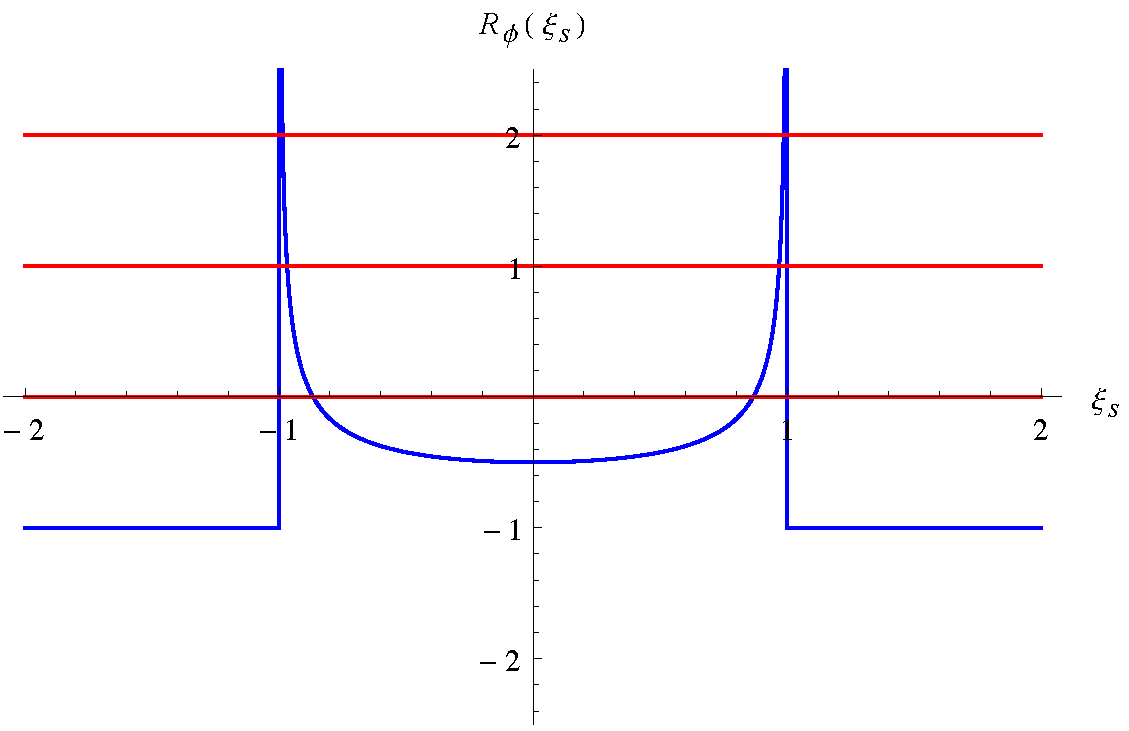
\includegraphics[scale=0.6]{Plots/ReRPhi.pdf}
\caption[Real part of the Regge trajectory function for the massless scalar exchange model]{Real part of $R_{\phi}(\xi_{s})$. The red lines correspond to $R_{\phi} = 0, 1, 2$. We have used $\alpha_{0} / m_{a} m_{b} = 0.5$.}
\label{ReRPhiFig}
\end{figure}

\begin{figure}
\centering
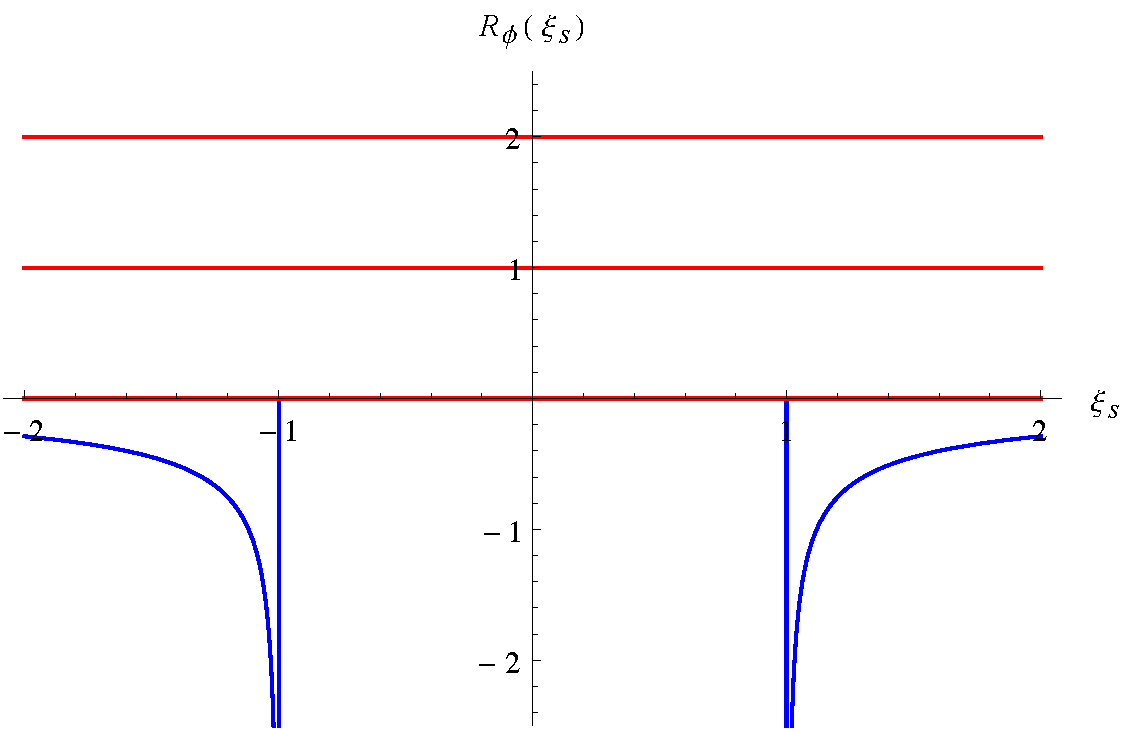
\includegraphics[scale=0.6]{Plots/ImRPhi.pdf}
\caption[Imaginary part of the Regge trajectory function for the massless scalar exchange model]{Imaginary part of $R_{\phi}(\xi_{s})$. The red lines correspond to $R_{\phi} = 0, 1, 2$. We have used $\alpha_{0} / m_{a} m_{b} = 0.5$.}
\label{ImRPhiFig}
\end{figure}
%%%%%%%%%%%%%%%%%%%%%%%%%%%%%%%%%%%%%%%%%%%%%%%%%%%%%%%%%%%%%%%%%%%%%%%%%%%%%%%%%%%%%%%%%
\subsubsection{Crossing}
%%%%%%%%%%%%%%%%%%%%%%%%%%%%%%%%%%%%%%%%%%%%%%%%%%%%%%%%%%%%%%%%%%%%%%%%%%%%%%%%%%%%%%%%%
Finally, a comment about crossing. The scattering event that we study is the elastic event
\begin{equation}
	a(p_{1}) + b(p_{2}) \longrightarrow a(p_{3}) + b(p_{4}) \label{sChannel}
\end{equation}
so the bound states are of the form $ab$. We can refer to (\ref{sChannel}) as the $s$-channel. If we cross the incoming $b$ particle with the outgoing $b$ particle, we find another elastic event
\begin{equation}
	a(p_{1}) + \bar{b}(\bar{p}_{2}) \longrightarrow a(p_{3}) + \bar{b}(\bar{p}_{4}) \label{uChannel}
\end{equation}
with
\begin{equation}
	\bar{p}_{2} = -p_{4}, \qquad \bar{p}_{4} = -p_{2}
\end{equation}
We can refer to (\ref{uChannel}) as the $u$-channel. In the $u$-channel the bound states are of the form $a \bar{b}$. This crossing amounts to switching $s$ with $u$. Note $\rho_{0}$ satisfies the functional relation $\rho_{0}(s, t) = \rho_{0}(u, t)$. That is, $\rho_{0}$ is invariant under crossing.

In the eikonal approximation we take $t \rightarrow 0$. Then $s$ and $u$ become eikonal-equivalent,
\begin{equation}
	s + u = 2m_{a}^{2} + 2m_{b}^{2}
\end{equation}
This relation allows us to perform an \textit{eikonal crossing}, where one replaces $s$ with $2m_{a}^{2} + 2m_{b}^{2} - u$ (instead of the usual crossing, where one replaces $s$ with $u$). The eikonal crossing is what enabled us to find the sequence (\ref{uJSca}) from (\ref{sJSca}). Under the eikonal crossing we have
\begin{equation}
	\xi_{s} = \frac{s - m_{a}^{2} - m_{b}^{2}}{2m_{a} m_{b}} = \frac{m_{a}^{2} + m_{b}^{2} - u}{2 m_{a} m_{b}} = - \xi_{u}
\end{equation}
But under the usual crossing we have
\begin{equation}
	\xi_{s} = \xi_{u}
\end{equation}
Since the Regge trajectory function is parity-symmetric, the same singularity condition must determine both the spectrum in the $s$-channel and the spectrum in the $u$-channel:
\begin{equation}
	R_{\phi}(\xi_{s}) = R_{\phi}(\xi_{u}) = R_{\phi}(-\xi_{s}) = R_{\phi}(-\xi_{u}) = J
\end{equation}
This property accounts for the apparent degeneracy in figure \ref{ReRPhiFig}.